\documentclass[convert={ghostscript,gsdevice=tiffg4,
outext=.tiff,density=1200}]{standalone}
    \usepackage{tikz}
    \usepackage{pgfplots}
    \usetikzlibrary{patterns}

\begin{document}
\Large
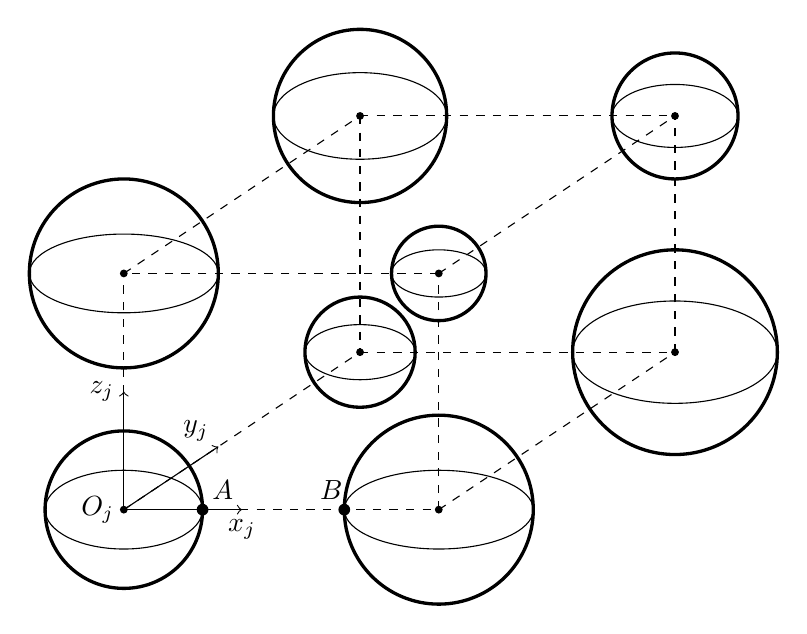
\begin{tikzpicture}%[scale=1.5]
\draw[->] (0,0) -- (1.2,0.8) node[anchor=north] {};
\draw[->] (0,0) -- (0,1.5) node[anchor=east] {$z_j$};
\draw[->] (0,0) -- (1.5,0) node[anchor=north] {$x_j$};

\node[left] at (0,0) {$O_j$};
\node[left] at (1.2,1) {$y_j$};
\node[above right] at (1,0) {$A$};
\node[above left] at (2.9,0) {$B$};

\draw[very thick] (0,0) circle (1.0);
\draw (0,0) ellipse (1.0 and .5);

\draw[very thick] (3,2) circle (0.7);
\draw (3,2) ellipse (0.7 and .35);

\draw[very thick] (0,3) circle (1.2);
\draw (0,3) ellipse (1.2 and .5);

\draw[very thick] (3,5) circle (1.1);
\draw (3,5) ellipse (1.1 and .55);


\draw[very thick] (4,0) circle (1.2);
\draw (4,0) ellipse (1.2 and .5);

\draw[very thick] (7,2) circle (1.3);
\draw (7,2) ellipse (1.3 and .65);

\draw[very thick] (4,3) circle (0.6);
\draw (4,3) ellipse (0.6 and .3);

\draw[very thick] (7,5) circle (0.8);
\draw (7,5) ellipse (0.8 and .4);

\draw[dashed] (0,0) -- (3,2);
\draw[dashed] (0,0) -- (0,3);
\draw[dashed] (3,5) -- (3,2);
\draw[dashed] (0,0) -- (4,0);
\draw[dashed] (0,3) -- (3,5);
\draw[dashed] (4,0) -- (4,3);
\draw[dashed] (4,3) -- (0,3);
\draw[dashed] (4,3) -- (7,5);
\draw[dashed] (4,0) -- (7,2);
\draw[dashed] (7,2) -- (7,5);
\draw[dashed] (3,2) -- (7,2);
\draw[dashed] (3,5) -- (7,5);

\node[circle, fill=black, inner sep=1pt] at (0,0) {};
\node[circle, fill=black, inner sep=1pt] at (3,2) {};
\node[circle, fill=black, inner sep=1pt] at (0,3) {};
\node[circle, fill=black, inner sep=1pt] at (3,5) {};

\node[circle, fill=black, inner sep=1.5pt] at (1,0) {};
\node[circle, fill=black, inner sep=1.5pt] at (2.8,0) {};

\node[circle, fill=black, inner sep=1pt] at (4,0) {};
\node[circle, fill=black, inner sep=1pt] at (7,2) {};
\node[circle, fill=black, inner sep=1pt] at (4,3) {};
\node[circle, fill=black, inner sep=1pt] at (7,5) {};

\end{tikzpicture}
\end{document}

%%% Local Variables: 
%%% mode: latex
%%% TeX-master: t
%%% End: 
